\documentclass[]{article}


% Title Page
\title{Kojo's Kitchen}
\author{Daniel de la Osa Fernandez\\ c412}


\begin{document}
\maketitle



\begin{section} {An\'{a}lisis de Kojo´s Kitchen}
La cocina de Kojo es uno de los puestos de comida r\'{a}pida en un centro comercial. El centro comercial está abierto entre las 10:00 am y las 9:00 pm cada d\'{i}a. En este lugar se sirven dos tipos de productos: s\'{a}ndwiches y sushi. Para los objetivos de este proyecto se asumir\'{a} que existen s\'{o}lo dos tipos de consumidores: unos consumen s\'{o}lo s\'{a}ndwiches y los otros consumen s\'{o}lo productos de la gama del sushi. En Kojo hay dos per\'{i}odos de hora pico durante un d\'{i}a de trabajo; uno entre las 11:30 am y la 1:30 pm, y el otro entre las 5:00 pm y las 7:00 pm. El intervalo de tiempo entre el arribo de un consumidor y el de otro no es homog\'{e}neo, pero por conveniencia, se asumir\'{a} que es homog\'{e}neo. El intervalo de tiempo de los segmentos homog\'{e}neos, distribuyen de forma exponencial con el par\'{a}metro $\lambda$ tal que como media los intervalos de llegadas entre clientes son la siguiente: 

\begin{center}
	\begin{tabular}{|c|c|c|} \hline
		Per\'{i}odo 	&  Intervalo de llegadas   $\lambda$ (mins)	 \\ \hline
		10:00-11:30 	& 16	 						\\ \hline
		11:30-13:30 	& 2								\\ \hline	
		13:30-17:00 	& 13							\\ \hline
		17:00-19:00 	& 3		 						\\ \hline 	
		19:00-21:00		& 10	 						\\ \hline 
	\end{tabular}
\end{center}

Actualmente dos empleados trabajan todo el d\'{i}a preparando s\'{a}ndwiches y sushis para los consumidores. El tiempo de preparaci\'{o}n depende del producto en cuesti\'{o}n. Estos distribuyen de forma uniforme, en un rango de 3 a 5 minutos para la preparaci\'{o}n de s\'{a}ndwiches y entre 5 y 8 minutos para la preparaci\'{o}n de sushi.

El administrador de Kojo est\'{a} muy feliz con el negocio, pero ha estado recibiendo quejas de los consumidores por la demora de sus peticiones. \'{E}l est\'{a} interesado en explorar algunas opciones de distribución del personal para reducir el número de quejas. Su inter\'{e}s est\'{a} centrado en comparar la situaci\'{o}n actual con una opci\'{o}n alternativa donde un tercer empleado durante los per\'{i}odos m\'{a}s ocupados. La medida del desempe\~{n}o de estas opciones estar\'{a} dada por el por ciento de consumidores que espera m\'{a}s de 5 minutos por un servicio durante el curso de un d\'{i}a de trabajo. 

\end{section}


\begin{section} {Ideas seguidas para la soluci\'{o}n}
Este problema es muy similar al problema de atender a clientes con n servidores en paralelo con la diferencia de que todo el tiempo no est\'{a}n disponibles estos servidores, en nuestro problema los cocineros. Los clientes comenzaran a a llegar a la cafeter\'{i}a a pedir s\'{a}ndwich o sushi con siguiendo una distribuci\'{o}n exponencial como indica el ejercicio.

Cuando un cliente llega uno de los cocineros lo atiende lo que equivale a generar el tiempo de salida del cliente del establecimiento. Esto se logra generando una variable aleatoria con distribuci\'{o}n uniforme(a, b) en dependencia si lo que quiere es s\'{a}ndwich o sushi, para saber que es lo que quiere el cliente se genera un v.a con distriuci\'{o}n bernoulli con p=0,5. Esto se podría variar en dependencia si las personas piden mas un producto u otro. 

Otro caso ser\'{i} cuando el cliente llegue y no hay ning\'{u}n cocinero disponible en este caso se coloca en una cola y hasta que llegue el tiempo de salida de alguno de los que se están atendiendo y entonces se le da su tiempo de salida, siempre que sea el primero de la cola sino solo se acerca m\'{a}s a ser atendido pero sigue encolado. Se defini\'{o} el tiempo de espera del cliente como el tiempo en que sali\'{o} de la cola menos el tiempo en el que llego al establecimiento.

Sea T el tiempo en el que el establecimiento cierra, todos los clientes que est\'{e}n en cola ser\'{a}n atendidos y los clientes que lleguen pasada esa hora no se dejar\'{a} que entren; as\'{i} el sistema podr\'{a} atender a los que falta y despu\'{e}s terminar.

Para el an\'{a}lisis que se pide la idea es trabajar con la media del tiempo de demora de los clientes en varios d\'{i}as de simulaci\'{o}n de la cocina de Kujo. Esta cantidad de d\'{i}as la puede definir el usuario pero de no ser así se simulan 30 días inicialmente y luego se utiliza una f\'{o}rmula estad\'{i}stica para saber si con esa cantidad de d\'{i}as es suficiente para estimar el par\'{a}metro que se quiere con un error previamente definido en este caso se tomo error de 1 minuto. La f\'{o}rmula utilizada fue (formula). Donde d=1, S es la ra\'{i}z del estimador puntual para la varianza y n = k la cantidad de d\'{i}as simulados hasta ese momento.    

\end{section}
                 


 
%Dentro de los elementos que hay que tener en cuenta es que los tiempos de los intervalos de llegadas de los clientes, que distribuyen de forma exponencial con parámetro lambda , este lambda fue tomado como 1/$\lambda$ para lograr tiempos en minutos mas realistas ya que la esperanza de la exponencial es 1/$\lambda$.                 

\begin{section} {Modelo}
	Aqu\'{i} se presentar\'{a} el modelo seguido para lograr la simulaci\'{o}n basada en eventos discretos donde las variables y los eventos toman un papel fundamental.  

\begin{subsection} {Estados}
	\begin{itemize}
		\item LLegada de un cliente a la cocina de Kujo
		\item Partida de un cliente que esta siendo atendido por el cocinero i  
	\end{itemize}
\end{subsection}

\begin{subsection} {Variables }
		\begin{itemize}
		\item t :			Tiempo actual en que se encuentra el sistema.
		
		\item T :	    	Tiempo en el cual cierra la tienda.
		
		\item n :			Cantidad de clientes totales que hay el sentido.
		
		\item nA: 			Cantidad de clientes que han llegado al sistema.
		
		\item cooks: 		N\'{u}mero de cocineros.
		
		\item ta: 			Tiempo de llegada.
		
		\item ti(i): 		Tiempo en que el cocinero i se desocupa.
		
		\item D(i):  		Tiempo de partida del cliente i.
		
		\item TimeInWait(i): Tiempo en que sale el cliente i de la cola. 
		
		\item $SS = (n, i1 , i2 ,... ,iN )$ (n clientes en el sistema, con i sub j  atendido por el cocinero j en este caso solo $j=(1,2,3)$. Si n$>$N los $n-N$ restantes est\'{a}n en cola). Si $S=(0)$ significa que el sistema est\'{a} vac\'{i}o. Si para algun i si $S[i]=0$ significa que el cocinero i esta disponible. 
		 	 	  		 
	\end{itemize}
\end{subsection}


\begin{subsection} {Inicializaci\'{o}n }
	\begin{itemize}
		\item $t0=600$ (Esto corresponde a las 10am en minutos).
		\item $T=1260$ (Equivale al tiempo de cierre)
		\item $ti=[infinity]*cooks$ 
		\item $ta=t0$
		\item demand interval =False  (Variable para indicar el cambio de intervalo de uno normal a otro critico importante cundo se simula con tres cocineros)

	\end{itemize}
	
\end{subsection}

\begin{subsection} {LLegada de Cliente}
	El primer caso que queremos ver es el arribo al sistema de un cliente esto siempre va a ejecutarse siempre que sea el tiempo mas cercano al actual(t) y que sea posible que llegue alguien es decir que $ta<T$.
	
	Al ocurrir esto se aumenta nA as\'{i} como n ya que llego alguien nuevo al sistema. Luego hay tres opciones el sistema est\'{a} vac\'{i}o, hay al menos un servidor vac\'{i}o o todos est\'{a}n llenos.
	
	Si ocurre lo primero hacer $SS = (1, nA , 0 ,0)$ (poner al cliente en el 1er cocinero) y generar su tiempo de salida y hacer $ti(0) = t +$valor generado 
	
	Si ocurre lo segundo se pone el cliente en el lugar del cocinero disponible. Tener en cuenta que si estamos en el caso de tres cocineros hay que revisar en que intervalo estoy, ya que si no es el cr\'{i}tico tienen que haber al menos dos disponibles ya que un cocinero va dejar de trabajar. De nuevo se genera el tiempo de salida del cliente que se comenz\'{o} a atender.
	
	Si ocurre el tercero pues se encola al cliente al final de SS y se aumenta SS[0] en uno.
	
	Luego se genera el pr\'{o}ximo arribo haciendo ta= t + valor generado 
	   
	
\end{subsection}

\begin{subsection} {Partida de un cliente del cocinero i}
	En este caso va a entrar si el tiempo de terminar que marca ti[i] es el pr\'{o}ximo en la lista de eventos en el tiempo es decir si es el menor de todos los posibles tiempos a moverse.
	
	Nos movemos a ese tiempo haciendo t=ti[i] disminuimos en 1 a n y hacemos también guardamos el tiempo de salida para el cliente que estaba siendo atendido por \'{e}l.
	
	Si el solo quedaba ese cliente en el sistema hacemos SS=[0] y ti[i]=infinito.
	Si no hay clientes en cola hacer cero la posici\'{o}n de SS correspondiente a ese cliente y poner ti[i]=infinito
	
	Si existen clientes en cola simplemente poner el pr\'{o}ximo de la cola en la posici\'{o}n de SS del cocinero que termin\'{o} y generar la salida de ese cliente para actualizar ti[i] al igual que se hace en el caso de entrada. Tener en cuenta que si es para tres cocineros pasa lo mismo de que si estas en un intervalos que no es de demanda entonces no se coloca ese cocinero a trabajar simplemente se hace cero en SS y se pone a infinito ti[i].
	   

	
	
\end{subsection}
\begin{subsection} {Caso cierre}
	Si no existe nadie en el sitema es decir n es igual a cero o SS=(0) y el pr\'{o}ximo tiempo a moverme es mayor que T pues termine el proceso de un d\'{i}a de simulaci\'{o}n 
	
	
	
\end{subsection}



\end{section}


\begin{section} {Resultados}
	Con este proyecto se logr\'{o} mediante una simulaci\'{o}n basada en eventos discretos describir el funcionamiento de la cocina de Kujo. La aplicaci\'{o}n nos permite generar simulaciones para la cantidad de d\'{i}as escogidos con intervalos de llegada de los clientes tamb\'{i}en modificables y en todos los casos el poner un nuevo cocinero resulto factible en disminuir el por ciento de clientes insatisfechos. Tamb\'{i}en jugar con los par\'{a}metros de entrada pueda dar otras informaciones como son la media de espera o la necesidad de que aunque con tres empleados es mejor para un flujo determinado puede ser aun insuficiente para lograr un mejor servicio a clientes. Ya que aunque esperan menos los clientes siguen esperando mucho tiempo para alg\'{u}n flujo de llegada x. Tamb\'{i}en la aplicaci\'{o}n permite la escalabilidad del negocio probando con nuevas configuraciones antes de crecer y as\'{i} aprovechar al maximo la inversi\'{o}n. Finalmente mostramos una salida del programa para 100 d\'{i}s con los lambdas por defecto.
	    
\end{section}
\begin{section} {Anexos}
	\begin{figure}
		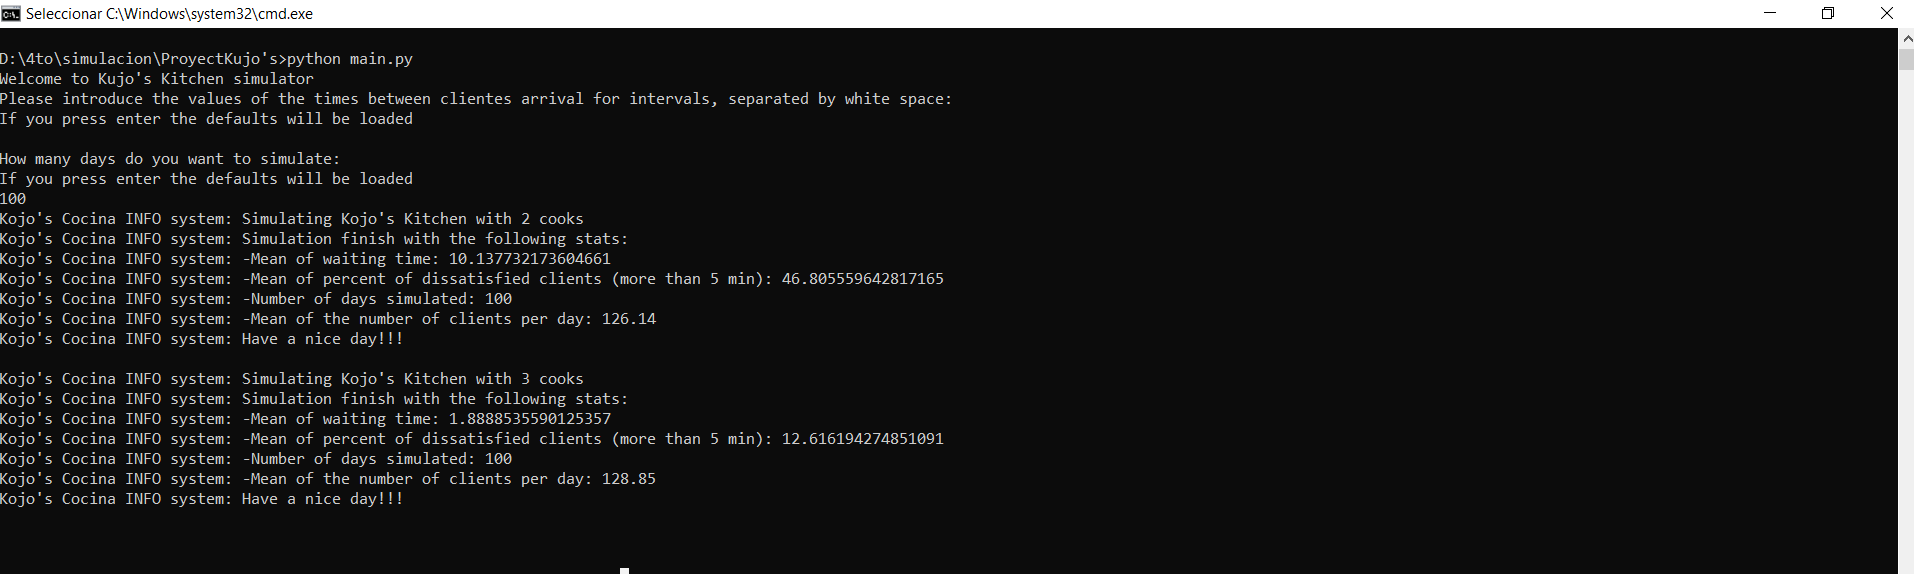
\includegraphics{Corrida.png}
		
		
		\caption{}
	\end{figure}
\begin{figure}
		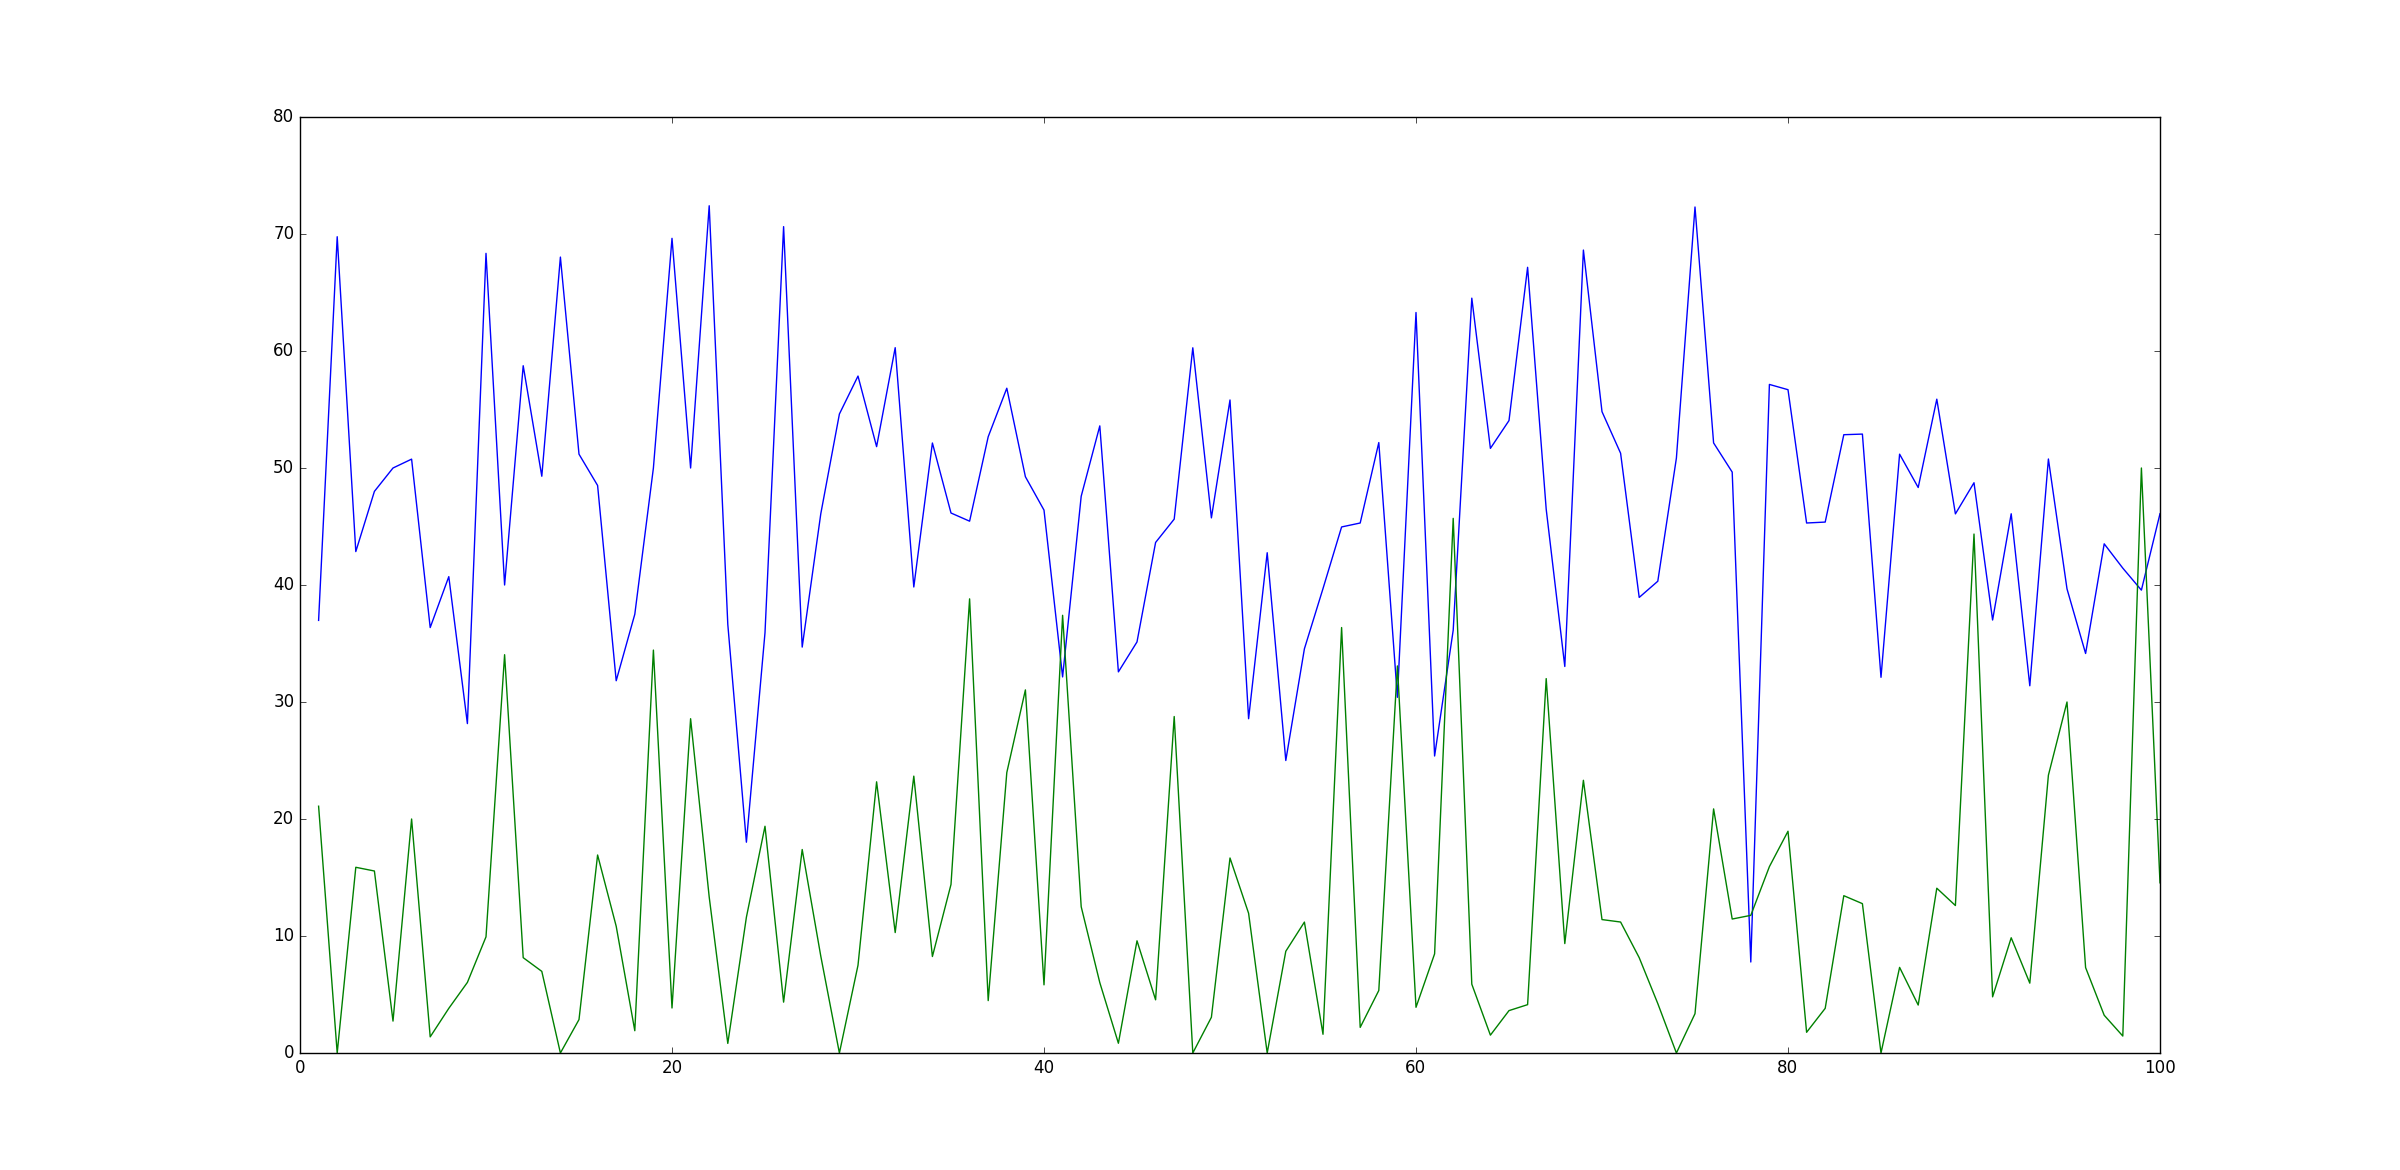
\includegraphics{figure_1.png}
	
	
	
	\caption{}
\end{figure}


	
\end{section}
	
\end{document}
